\documentclass{article}

\usepackage{geometry}
 \geometry{
 a4paper,
 left=25mm,
 right=20mm,
 top=20mm,
 }

\usepackage{exercise}
\usepackage{enumerate}
\usepackage{graphicx}
\usepackage{subfig}
\usepackage{listings}

\graphicspath{ {images/} }

\lstset{language=python, firstline=37, lastline=45, title={Listing 1: Data structures for cellular automaton}}

\begin{document}

\title{
Computational Geometry and Digital Images \\
fork-recognition\\
Project report
}

\author{Etienne Moutot, Ievgeniia Oshurko}
\date{April 6, 2016}
\maketitle


\section{Introduction}  

\section{Feature Engineering}
\subsection{Medial Axis}

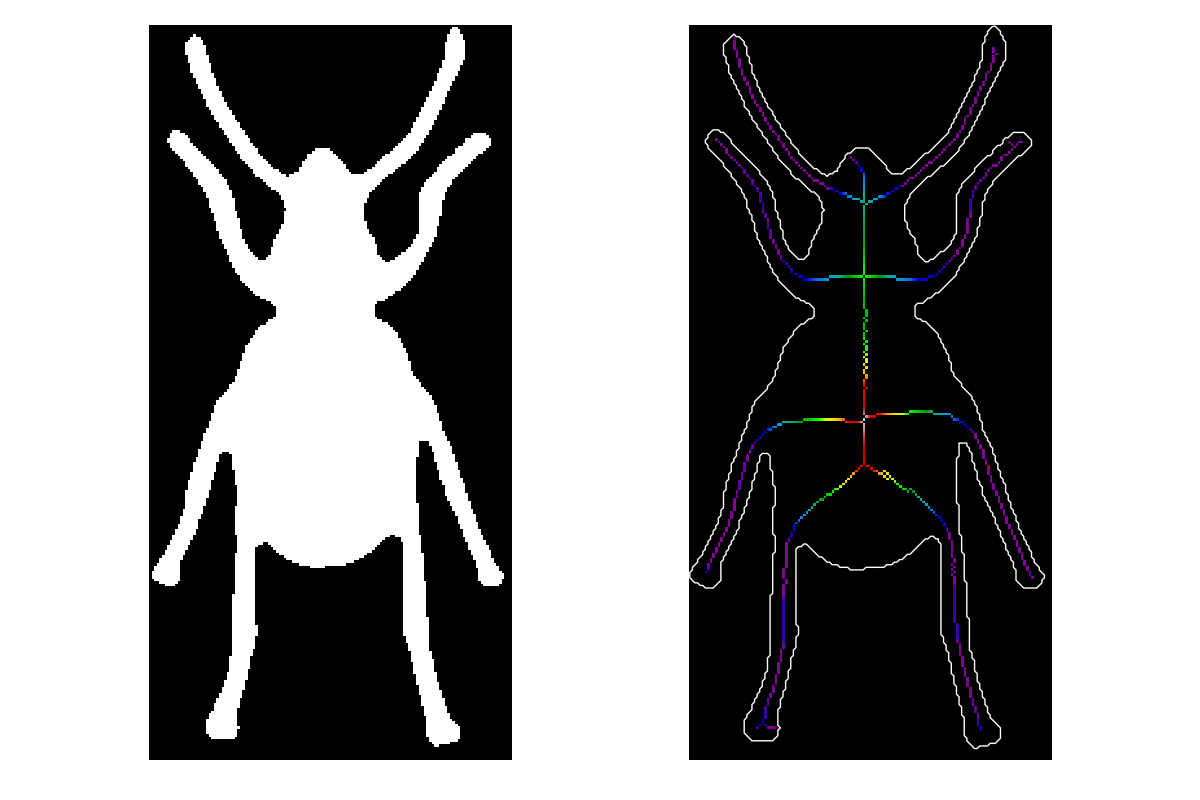
\includegraphics[scale=0.25]{beetle_281.png}
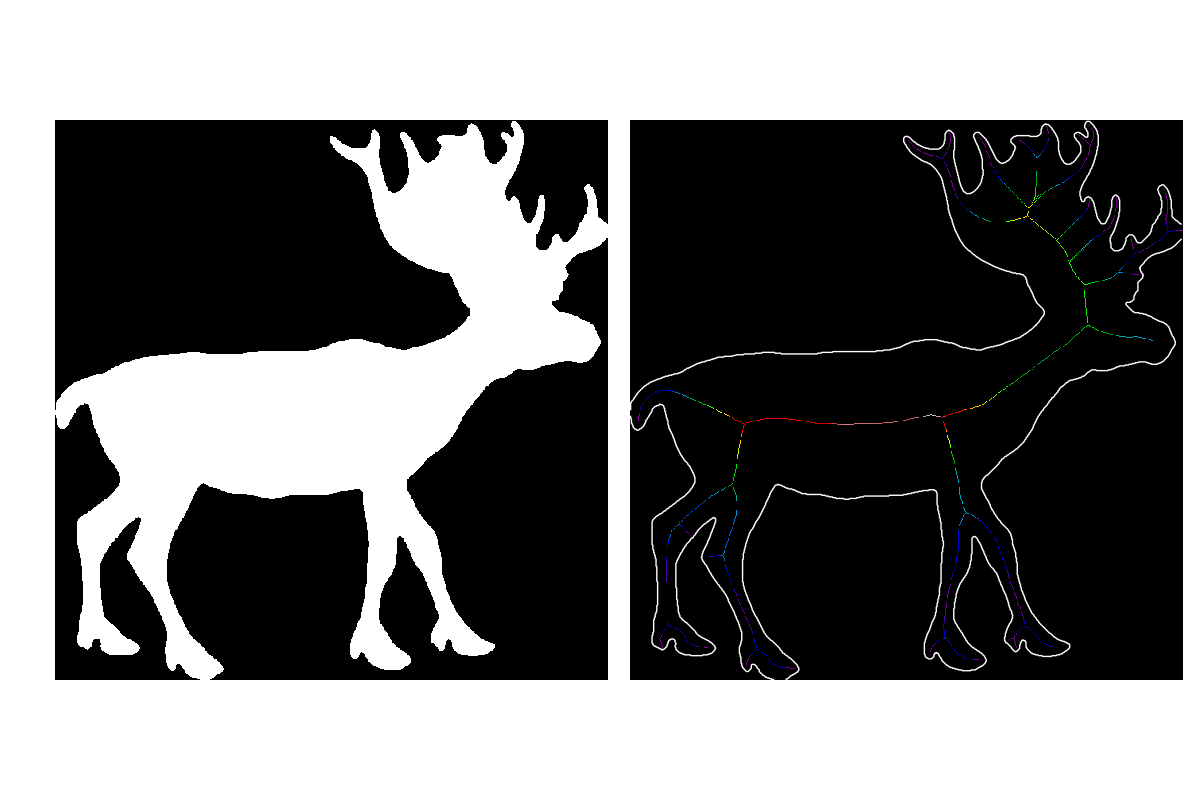
\includegraphics[scale=0.25]{deer_79.png}

\vspace{12px}

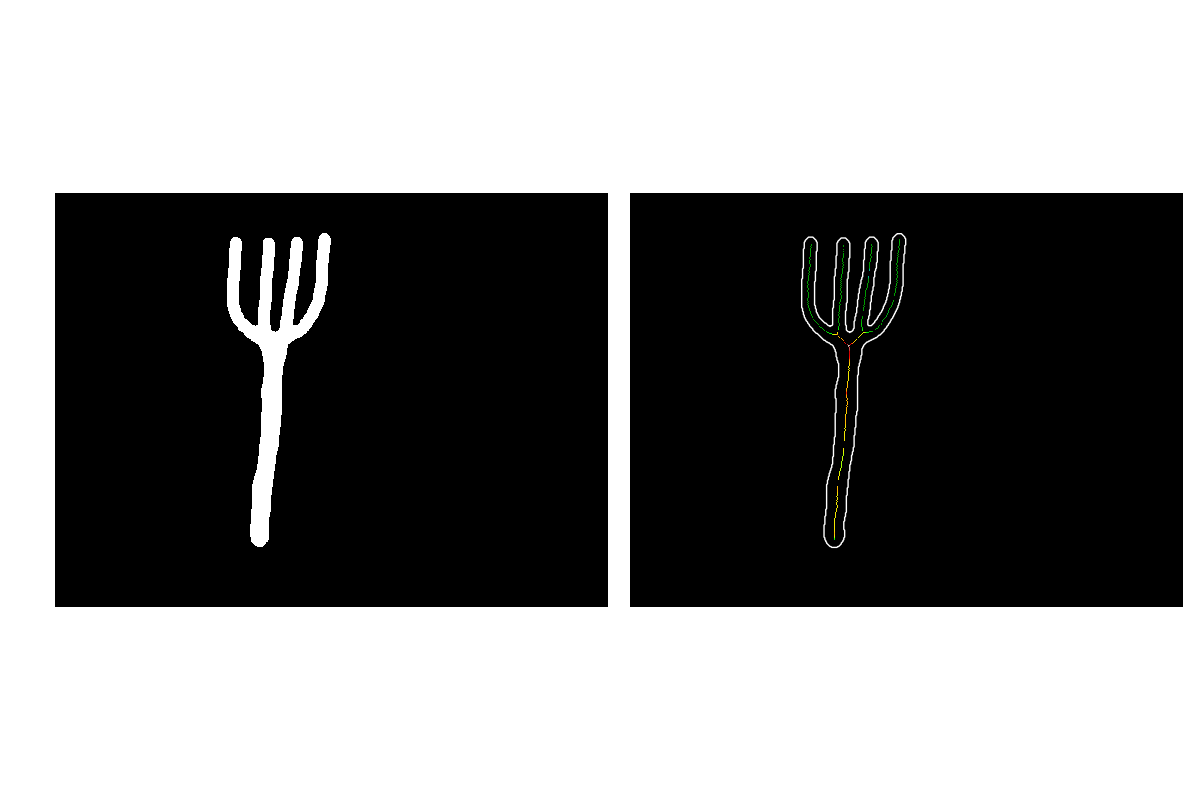
\includegraphics[scale=0.25]{fork_75.png}
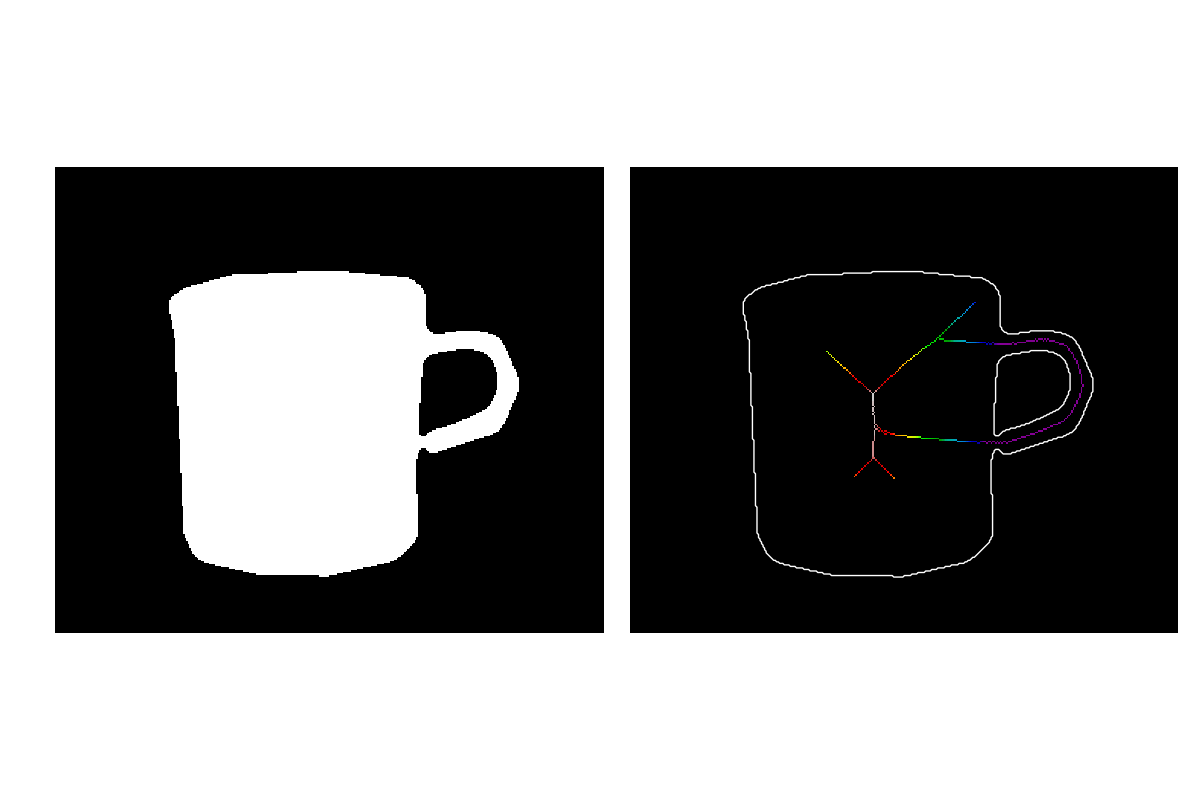
\includegraphics[scale=0.25]{cup_476.png}


\subsubsection{Histogram of distance of the medial axis points from borders}
\subsubsection{Histogram of length of the medial axis straight lines}
\subsubsection{Quantitive features of skeleton}

\subsection{Border Curvature}
\subsubsection{Histogram of border curvature coefficients}

\subsection{Volumetric Features}
\subsubsection{Scaled area}
\subsubsection{Solidity and extend}
\subsubsection{Scaled major and minor axes length}
 
\section{Classification models}
\subsection{Gaussian Naive Bayes}
\subsection{K Nearest Neighbours}

\section{Results and Discussions}
\subsection{Performance}
\subsection{Robustness and scale/rotation invariance}
\subsection{Conclusions}

\end{document}
